\chapter{Bonding}
\section{Introduction}
\subsection{Topics}
\begin{enumerate}
  \item Lewis dot structures
  \item Molecular geometry
  \item Resonance
  \item Formal charge
  \item Polarity
  \item Hybrid orbital theory
\end{enumerate}

\subsection{Bond Types}
\begin{description}
  \item[Ionic bonding] electrons are removed from one atom and donated to
    another.
  \item[Covalent bonding] electrons are shared in well-defined spaces between
    atoms.
  \item[Metallic bonding] orbitals of atoms overlap.
\end{description}

\section{Lewis dot structures}
\subsection{Counting valence electrons}
Valence elecftrons respresnt the outside surface of an atom. It is the outermost
or highest energy-level of the electron shell. These numbers can be easily
obtained from the periodic table, and inserted into the below electron
"template":

$$1s^22s^22p^63s^23p^64s^23d^104p^6 \ldots$$

\begin{description}
  \item[s-block] The row number is the highest energy level.
  \item[d-block] $\text{row}-1$ is the highest energy level.
  \item[p-block] Use noble gases.
\end{description}

\subsection{Drawing}
Lewis dot structures just show the valence electrons present in an atom.

\subsubsection{Single atoms}
For single atoms, the electrons are placed above, below, to the left or right of
the element symbol. Electrons should not be paired until each spot has an
electron present.

\lewis{0.4.,Be}

\subsubsection{Ionic bonding}
Place species in a box, show the charge outside the box.

\lewis{0.,Na}

$\chemleft[\lewis{,Na}\chemright]^{+}$

\subsubsection{Covalent bonding}
\chemfig{Cl(-[:0]F)(-[:90]O)(-[:180]H)(-[:270]F)}

\subsection{Octet rule}
The octet rule says that, for the majority of atoms, a stable molecule is formed
when each atom has eight electorns available to it.

There are a few exceptions to this rule, however:
\begin{enumerate}
  \item \ce{H} only needs two electrons to fill its valence level, so it only
    needs two electrons near it to form covalent bonds.
  \item \ce{B} can be stable with either eight or six electrons, six being the
    more common form.
  \item \ce{Be} sometimes forms covalent bonds. It only needs four electrons to
    do this.
  \item \ce{P}, \ce{S}, and \ce{Cl} (as well as all elements below them on the
    table) can have eight or more valence electrons. These atoms do not form
    double or triple bonds to break the octet rule, but will exceed an octet as
    they form single bonds.
\end{enumerate}

\section{Bond properties}
The sharing of multiple pairs of electrons can result in higher-order bonding.
four shared electrons results in a double bond, six in a triple. Quadruple bonds
are not considered on this exam.

In general: as the number of electrons shared between atoms increases, the
strength increases and the distance between atoms decreases.

\section{Lewis structures (again)}
In general, to draw a lewis structure, implement the following processes:

\begin{enumerate}
  \item Determine the central atom. \ce{H} will never be the central atom, the
    the atom with the lowest electronegativity usually will be.
  \item Count the total number of valence electrons for the group. If there is a
    charge, add or subtract electrons as necessary.
  \item Put the center atom in t he center and distribute other atoms around it
    with a single bond.
  \item Add electrons to the terminal atom such that each atom has an octet
    (except \ce{H}.
  \item Check that the center atom has (at least) an octet. If there are any
    unused electrons, they shall be placed on the center atom. If the center
    atom is short of an octet, double or triple bonding will be necessary.
\end{enumerate}

Some examples follow below:

\begin{description}
  \item[\ce{HCN}] \chemfig{C(-[4]H)(~[0]\lewis{0:,N})}
  \item[\ce{NH4^+}]
    $\chemleft[\chemfig{N(-[0]H)(-[2]H)(-[4]H)(-[6]H)}\chemright]^{1+}$
  \item[\ce{CO3^2-}]
    $\chemleft[\chemfig{C(=[0]\lewis{2:6:,O})(-[4]\lewis{2:4:6:,O})(-[6]\lewis{0:4:6:,O})}\chemright]^{2-}$
    $\chemleft[\chemfig{C(-[0]\lewis{0:2:6:,O})(=[4]\lewis{2:6:,O})(-[6]\lewis{0:4:6:,O})}\chemright]^{2-}$
    $\chemleft[\chemfig{C(-[0]\lewis{0:2:6:,O})(-[4]\lewis{2:4:6:,O})(=[6]\lewis{0:4:,O})}\chemright]^{2-}$
\end{description}

\section{Resonance structures}
If a double or triple bond is present and can exist in more than one location, a
resonnance structure is necessary. A resonnance structure is composed of several
lewis structures and displays all possible locations for the changing bond to be
placed. An example is shown below:

$\chemleft[\chemfig{C(-[:0]O)(-[:90]O)(=[:180]O)}\chemright]^{2-}$
$\chemleft[\chemfig{C(-[:0]O)(=[:90]O)(-[:180]O)}\chemright]^{2-}$
$\chemleft[\chemfig{C(=[:0]O)(-[:90]O)(-[:180]O)}\chemright]^{2-}$

\section{Formal charge}
Formal charge describes the change in electron distribution as a result of
covalent bonding.

\begin{equation}
  \text{Formal charge} = n_{valence} - (n_{unbonded} + \frac{1}{2}n_{shared})
\end{equation}

\section{Bond polarity}
Bond polarity represents an electronegativity differential between two atoms in
a shared bond and is used to determine the bond type.

\begin{equation}
  \text{polarity} = \chi_A - \chi_B
\end{equation}

\begin{table}[]
\centering
\begin{tabular}{l|l|l|l|l|l|l|l|l|l|l|}
\hline
\multicolumn{1}{|l|}{\textbf{Polarity}}              & 0.00                           & 0.65 & 0.94 & 1.19 & 1.43 & 1.67 & 1.91  & 2.19 & 2.54 & 3.03 \\ \hline
\multicolumn{1}{|l|}{\textbf{\% Ionic Character}}    & 0                              & 10   & 20   & 30   & 40   & 50   & 60    & 70   & 80   & 90   \\ \hline
\multicolumn{1}{|l|}{\textbf{\% Covalent Character}} & 100                            & 90   & 80   & 70   & 60   & 50   & 40    & 30   & 20   & 10   \\ \hline
                                                     & \multicolumn{1}{c|}{Non-polar} & \multicolumn{5}{c|}{Polar}       & \multicolumn{4}{c|}{Ionic} \\ \cline{2-11}
\end{tabular}
\end{table}

\section{Bond order}
Bond order represents the average bond strength over time between two given
atoms in a given molecule.

\begin{description}
  \item[Without resonance] The number of bonds between two atoms
  \item[With resonance] The mean number of bonds between two atoms in all
    structures
\end{description}

\section{Bond energy}
To predict the energy change of a reaction, it is possible to estimate the heat
of the reaction by examining the energy need to form and break all of the bonds.

For these equations, we let $D$ represent the energy needed to break one
particular bond.

\begin{equation}
  \Delta H_{rxn} = \sum_{i=1}^{n} n_iD_{broken} - \sum_{i=1}^{n} n_iD_{formed}
\end{equation}

\section{VSEPR Theory}
VSEPR theory is the "Valence Shell Electron-Pair Repulsion" theory and states
two main ideas:

\begin{enumerate}
  \item Atoms to the central atom should be spaced out as much as possible.
  \item Unbonded electron pairs should be spaced out as well, taking up slightly
    more space than a bond would.
\end{enumerate}

Electron-pair geometries show all spaced objects, containing both bonded atoms
and unbonded pairs.

Molecular geometries show only the bonded atoms distributed in space.

\subsection{VSEPR Geometries}
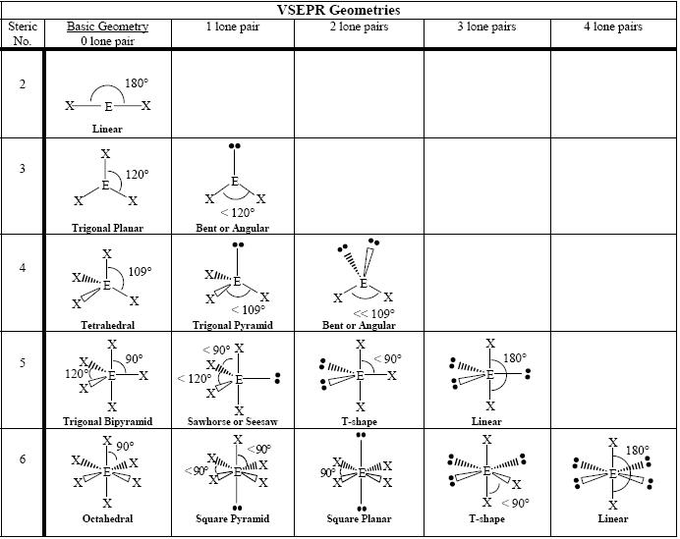
\includegraphics[width=\textwidth]{resources/vsepr-table.png}

\subsection{Polarity}
The "polarity" of a molecule refers to a vector of charge flowing throughout.
The polarity of a molecule depends on the polarity of the bonds in the molecular
geometry.

There is a distinction between the molecular diople and the individual component
bond dipoles that is illustrated below.

\begin{equation}
\vec{\mu}_{\text{mol.}} = \sum_{i=1}^{n} \vec{\mu}_{i}
\end{equation}

To determine the polarity of a molecule, implement the following processes:

\begin{enumerate}
  \item Draw a Lewis structure.
  \item Determine the molecular geometry.
  \item Determine the polarity of the individual bonds. (Positive points to
    negaitve).
  \item Draw bond dipoles as vectors.
  \item Sum the vectors and draw the molecular dipole.
\end{enumerate}

\subsection{Hybridization}
Orbitals on a single atom will hybridize to form new orbitals. These hybridized
orbitals will be combinations of valence level orbitals, which determines the
shape of a molecule.

Some hybridizations are listed below.

\begin{table}[]
\centering
\begin{tabular}{|l|l|l|}
\hline
\textbf{electron pair geometry} & \textbf{orbitals} & \textbf{hybridization} \\ \hline
linear                          & $s,p$             & $sp$                   \\ \hline
trigonal planar                 & $s,p,p$           & $sp^3$                 \\ \hline
tetrahedral                     & $s,p,p,p$         & $sp^3$                 \\ \hline
trigonal bipyramidal            & $s,p,p,p,d$       & $sp^3d$                \\ \hline
octahedral                      & $s,p,p,p,d,d$     & $sp^3d^2$              \\ \hline
\end{tabular}
\end{table}
